\thispagestyle{fancy}
% Leave Left and Right Header empty.
\lhead{}
\rhead{}
\renewcommand{\headrulewidth}{1pt}
\renewcommand{\footrulewidth}{0pt}
\fancyfoot[C]{}

\pagestyle{fancy}
\lhead{\bf Project Abstract}
\rhead{\bf Steven A. Rodney, University of South Carolina}

Within the next decade, NASA will be operating two new flagship
missions for space-based astronomical research.  The James Webb Space
Telescope (JWST) will launch in 2018, providing a new infrared
observatory that will be a powerful successor to the Hubble Space
Telescope (HST).  In the mid-2020's the Wide Field Infrared Survey
Telescope (WFIRST) will add an unprecedented new ability for wide-area
sky surveys from space.  Both of these telescopes will open up new
avenues for the study of stellar explosions (supernovae)---particularly
explosions from the very early universe that are currently too distant
and too faint for even HST to observe.

With JWST we will be able to see the peculiar supernovae that occurred
when the very first generation of stars died.  This glimpse at the
earliest epoch of star formation (and stellar death) will address
fundamental questions about the formation and early evolution of
galaxies and stars. Although WFIRST will not reach as deep into the
murky past, it will execute wide and fast surveys that will enable
detection of rare stellar explosions that occur in unusual places,
such as supernovae that happen to lie behind dense dark matter
clusters.  As sketched in Figure 1, a dense concentration of dark
matter between us and the supernova can act as a {\it gravitational
lens,} distorting and focusing the light from the background
supernova.  By measuring these effects we can learn about the
intervening dark matter or the nature of dark energy.

{\bf We propose to develop a new open-source software suite to
  simulate JWST and WFIRST supernova surveys,} implementing for the
first time a rigorous treatment of both gravitational lensing and the
peculiar stellar explosions that are unique to the early universe.  We
will then use these tools to design and evaluate the first supernova
surveys with JWST and WFIRST.  These simulations are {\bf necessary}
to efficiently allocate telescope resources and to properly account
for selection biases that would otherwise skew the interpretation of
very distant supernova samples.  This work is also {\bf timely}, as
our products will be available just in time for use in proposing for
JWST observing in 2019, and will be able to influence the ongoing
WFIRST mission design.  We plan to develop this software in the open,
making it instantly and {\bf widely accessible}.


\begin{figure*}[b!]
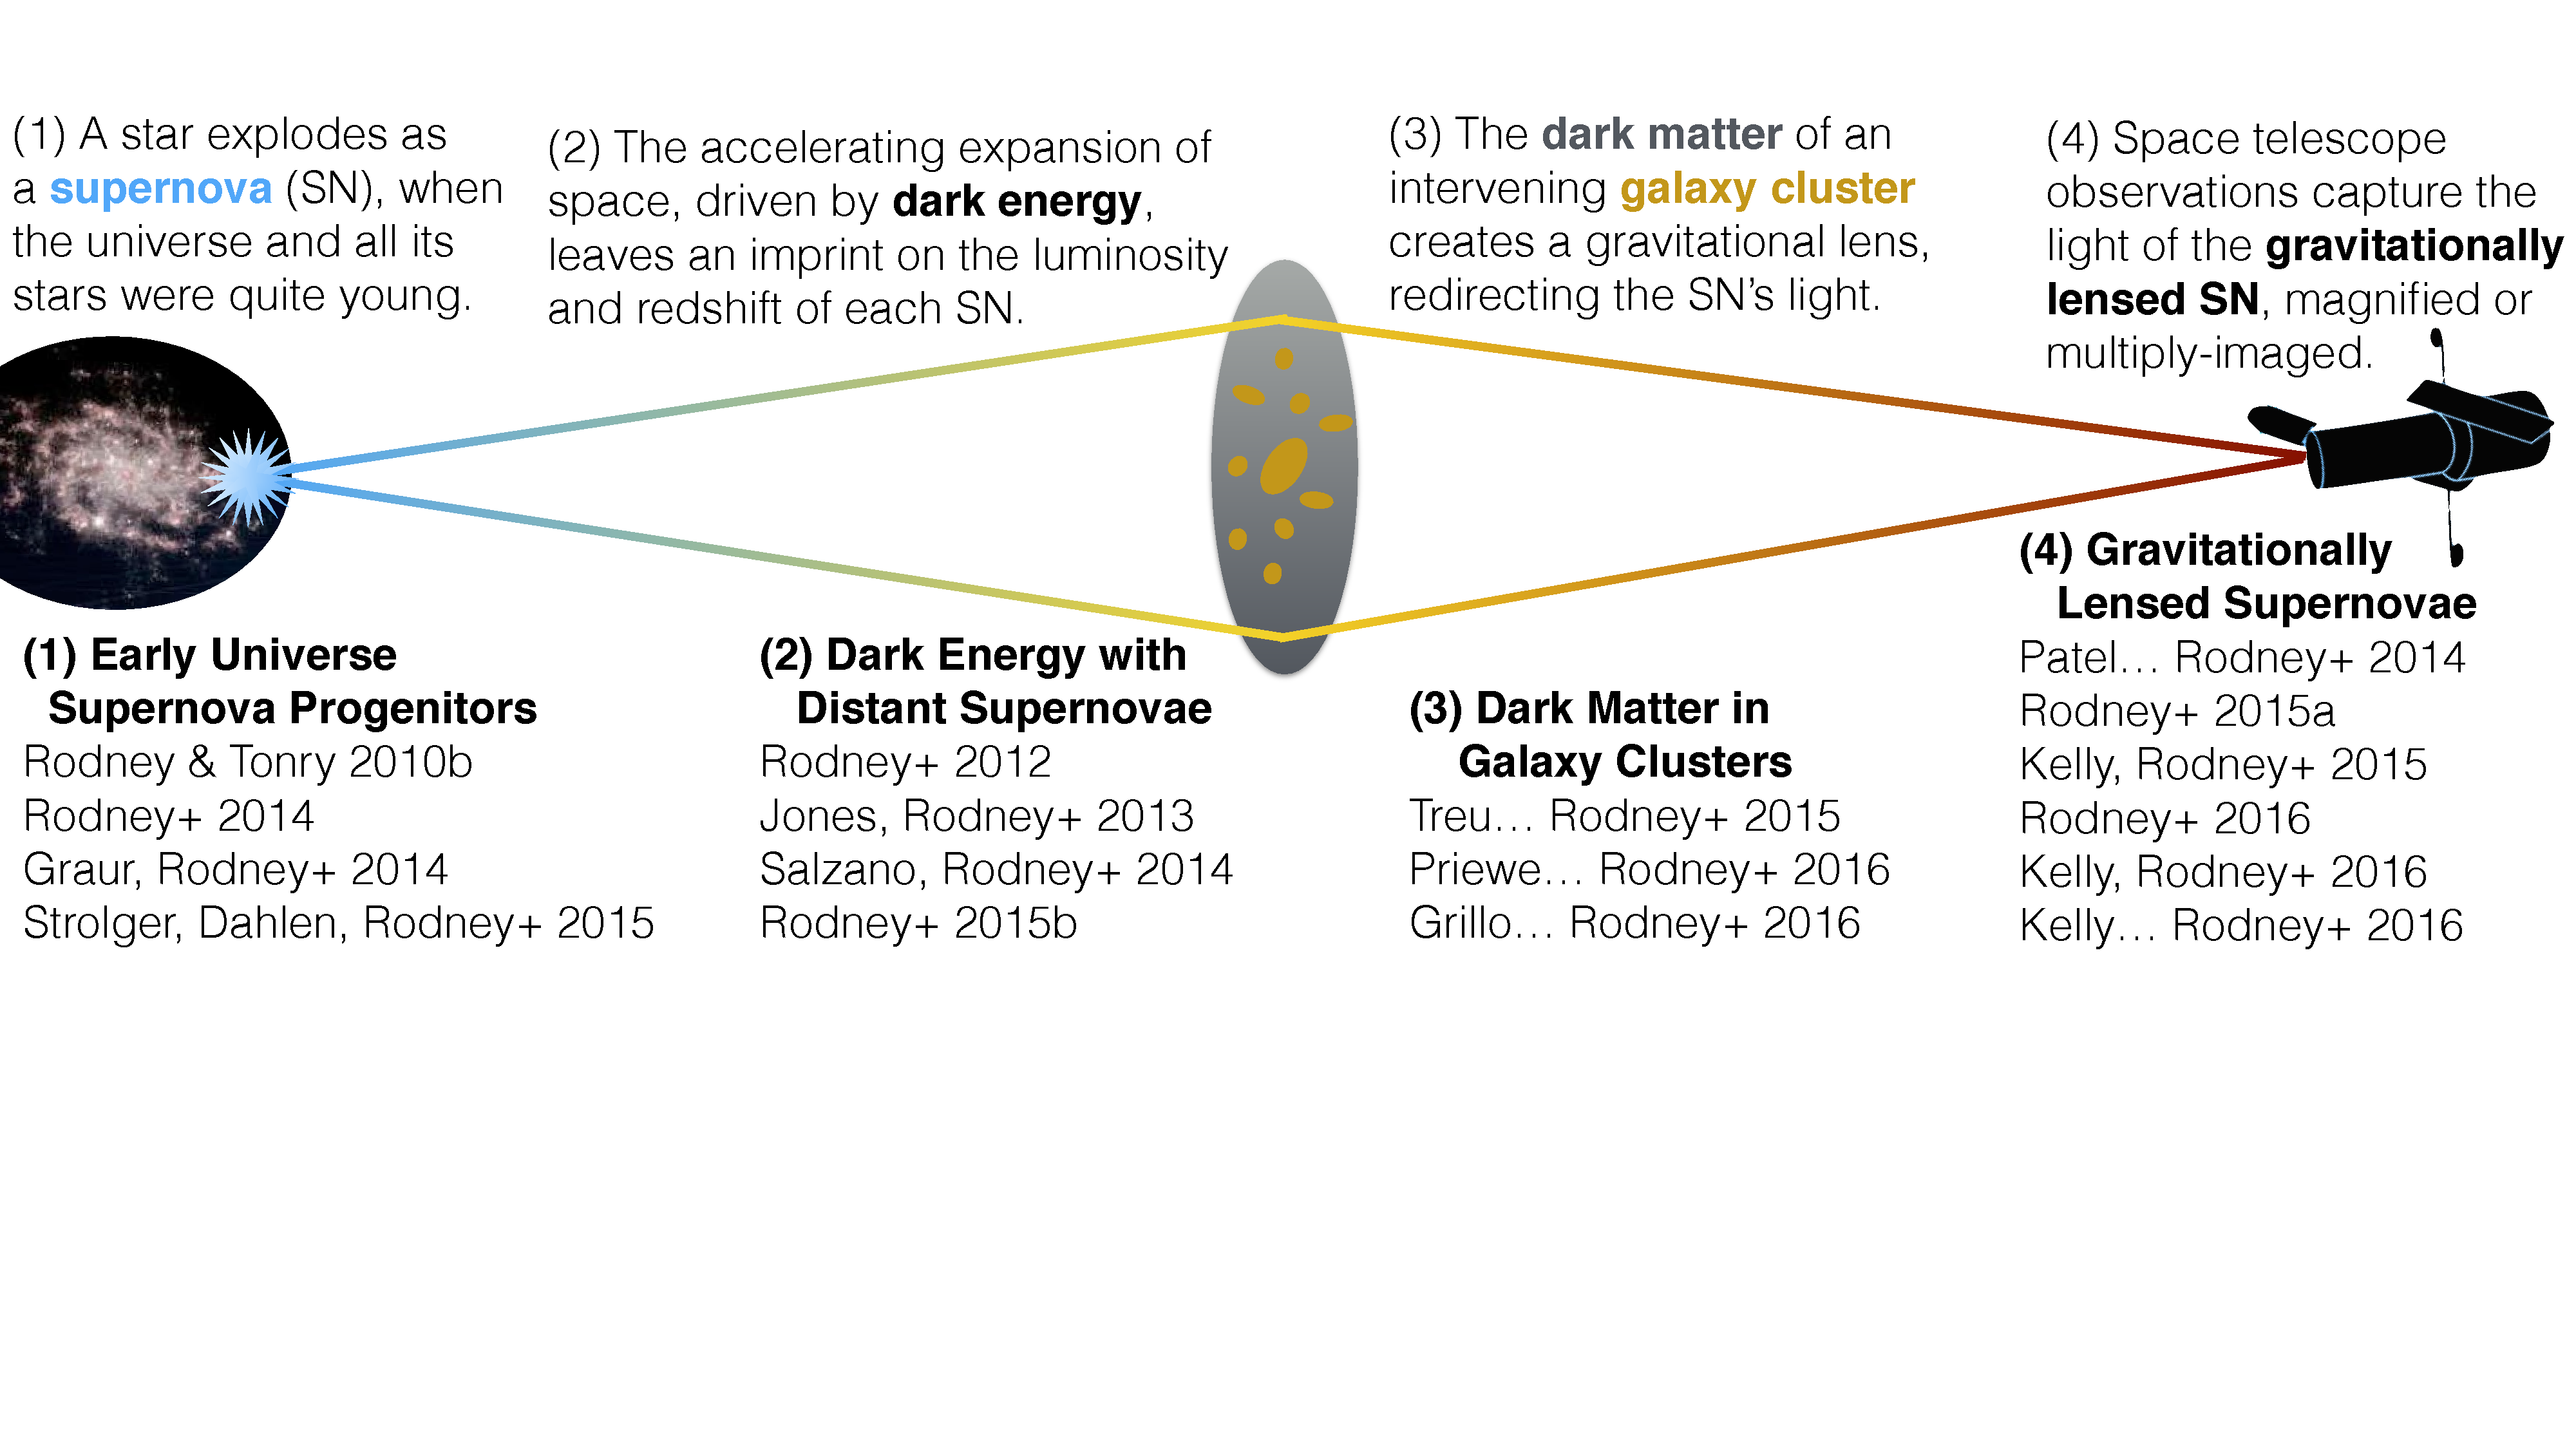
\includegraphics[width=\textwidth]{sloan_fellowship_fig.pdf}
\caption{
The context of supernova research led by PI Rodney.  This proposal
would develop new software that is relevant for all four branches of
the research program depicted here.}
\end{figure*}

